\documentclass[a4paper]{article}

\usepackage{amsmath}
\usepackage{amsfonts}
\usepackage{amssymb}
\usepackage[pdftex]{graphicx}
\usepackage[spanish]{babel}

%Mejoras: 1) Mejorar Bibliografía y ponerle referencias cruzadas.

\begin{document}

\begin{center}

\begin{center}
\includegraphics[scale=0.05]{Logo.PNG} 
\end{center}
\hspace{10pt}

\huge
\textbf{Modelado Perfil Térmico HRSG}\\ 

\Large
Tema de Trabajo Profesional - Rama Termomecánica\\ 

\hspace{10pt}

\large
\textit{Tutor: Ing. Pablo Barral}\\

\small
67.04 Termodinámica IA\\
67.33 Tecnología del Calor\\

\hspace{8pt}

\small  
\texttt{pbarral@fi.uba.ar}\\

\end{center}

\hspace{8pt}

\begin{center}
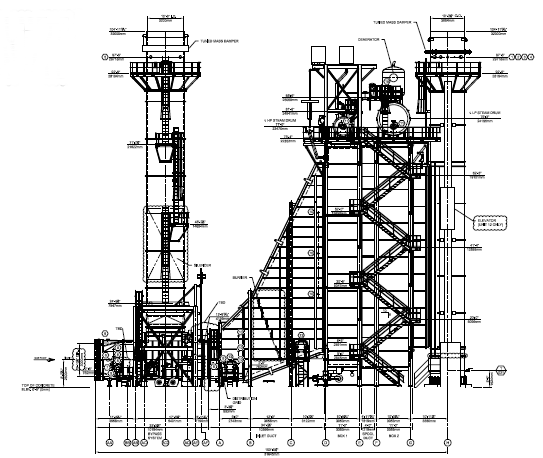
\includegraphics[scale=0.5]{Captura.PNG} 
\end{center}
\hspace{8pt}

\begin{flushright}
\textit{\today}
\end{flushright}

\newpage
\normalsize

\section*{Objetivos}

Los objetivos de este trabajo son desarrollar un modelo que permita simular el comportamiento del perfil térmico de una Caldera de Recuperación existente en particular con condiciones de borde distintas a la de diseño y extraer lineamientos para una metodología general.

\section*{Justificación}

Debido a diversos factores, hoy en día no hay en los generadores de energía eléctrica y en los cogeneradores un departamento dedicado a un análisis de los parámetros de operación desde un punto de vista térmico (sopesando el impacto de los parámetros en la potencia y el consumo específico). Esta carencia provoca una operación ciega, de poco poder predictivo y sin una cuantificación de la merma de la eficiencia provocada por cada fenómeno.

Para poder realizar el análisis de los datos de operación contra los de proceso es necesario construir una referencia comparable a partir de características constructivas de los equipos. Si bien existe un potente software comercial en la temática (la suite \textit{Thermoflow}, desarrollada por profesionales egresados del MIT), este es cerrado y no se puede acceder libremente a las ecuaciones que estipula para el modelado, limitando el campo de acción del ingeniero de proceso. También los fabricantes otorgan los datos de performance esperada. Sin embargo, sólo lo hacen para casos particulares y resulta deseable poder realizar esta tarea con independencia y con condiciones de borde a priori desconocidas.

Por otra parte, conocer el comportamiento de una caldera de recuperación en distintas situaciones permite realizar estudios de factibilidad de cogeneraciones más representativos y refinados, en casos con curvas anualizadas de demanda, en lugar de escenarios estáticos.

Asimismo, resulta interesante poder continuar y ampliar la línea de trabajo comenzada en el año 2015 por un grupo de profesionales del Departamento con especialistas españoles y mexicanos. Línea en la que, además, no se encuentra trabajando nadie en el país.

Finalmente, sostenemos que este trabajo permitirá a alumnos avanzados de la carrera de Ingeniería Mecánica conocer el detalle constructivo de de un equipo principal de una central térmica, sus parámetros de proceso, su filosofía de control, así como bibliografía especializada y el uso de herramientas informáticas comunes en el área.

\section*{Metodología del Trabajo}

Se propone la realización de una ingeniería inversa sobre una Caldera de Recuperación (HRSG) existente de un fabricante reconocido: utilizando como base los datos de performance de diseño, seleccionar y aplicar una serie de correlaciones presentes en la bibliografía entre la transferencia de calor, la pérdida de carga y la geometría al caso de estudio elegido, eligiendo entre ellas las que presenten mejor ajuste al caso en particular y modificándolas en caso de ser necesario. 

Para dicha aplicación se trabajará en la construcción de un simulador informático utilizando el software \textit{Engineering Equation Solver}, que se encuentra disponible. Este tiene la capacidad de resolver ecuaciones no lineales como las termodinámicas y cuenta con una amplia biblioteca de funciones de estado. No serán realizados estudios CFD.

\section*{Relación con otros Trabajos}

Este trabajo tiene como antecedentes el Trabajo Profesional (en colaboración) del tutor, basado en desarrollos de especialistas españoles del Instituto CIRCE de la Universidad de Zaragoza y el curso sobre Diagnóstico de Ciclos Térmicos Complejos dictado en la Facultad, en conjunto con un especialista mexicano en la temática.

Estos trabajos estuvieron focalizados en métodos de comparación entre operación y referencia, utilizando modelos totalmente ad hoc (una extrapolación totalmente numérica) para poder construirla, por limitaciones en la génesis de los proyectos.

En paralelo, se prevé la propuesta de un Trabajo Profesional análogo para el comportamiento de otro de los equipos principales de un ciclo combinado o cogeneración: la Turbina de Vapor. 

Una vez concluidos ambos servirán como precedente de una tercera propuesta: la aplicación, en Argentina, del desarrollo del especialista mexicano a un caso real.

\newpage
\section*{Bibliografía}

\begin{enumerate}
%\item Author, A. (Year of Publication). \textit{Title of work.} Publisher City, State: Publisher.

\item Rezaie Navaie, A. (2017). \textit{Thermal Design and Optimization of Heat Recovery Steam Generators and Waste Heat Boilers.} Disertación. Berlín: Technische Universität Berlin.

\item Barral, P., Rinaldi, G., y Sapollnik, A. (2017). \textit{Diagnóstico Termoeconómico de Plantas de Generación.} Trabajo Profesional de Ingeniería Mecánica, rama termomecánica. Buenos Aires: Facultad de Ingeniería, Universidad de Buenos Aires.

\item Verein Deutscher Ingenieure - Gesellschaft Verfahrenstechnik und Chemieingenieurwesen (2010). \textit{VDI Heat Atlas.}(2ª ed.) Berlin: Springer-Verlag.

\item Kreith, F. (Ed.) (2000). \textit{The CRC Handbook of Thermal Engineering.} Boca Raton, FL: CRC Press.

\item Bejan, A. (2013). \textit{Convective Heat Transfer.}(4ª ed.) Hoboken, New Jersey: John Wiley \& Sons, Inc.

\item Bejan, A., y Kraus, A. (2003). \textit{Heat Transfer Handbook.} Hoboken, New Jersey: John Wiley \& Sons, Inc.

\item Klein, S., y Nellis, G. (2009). \textit{Heat Transfer.} New York: Cambridge University Press.

\item Klein, S., y Nellis, G. (2012). \textit{Thermodynamics.} New York: Cambridge University Press.

\item Klein, S., y Nellis, G. (2012). \textit{Mastering EES.} Madison, Wisconsin: F-Chart Software.

\item Ganapathy, V. (2015). \textit{Steam Generators and Waste Heat Boilers: For Process and Plant Engineers.} Boca Raton, FL: CRC Press.

\item Eriksen, V. (Ed.) (2017). \textit{Heat Recovery Steam Generator Technology.} Duxford: Woodhead Publishing.

\item Kitto, J., y Stultz, S. (Ed.)  (2005). \textit{Steam/its generation and use.}(41ª ed.) Barberton, Ohio: The Babcock \& Wilcox Company.

\end{enumerate}
\end{document}